A range query is a database operation that retrieves all the records that lies in a range. In this project, we perform range query on 2-dimension data only. In addition, we only consider a range query where the range is defined as a rectangle. Under these assumptions, a range query can be formalised as a query $\mathcal{Q}(\boldsymbol{l}, \boldsymbol{u})$ where $l,u\in\mathbb{R}^2$.

\begin{mscexample}
	For example, assume we have the points
	$$
	[(1,2), (3,4), (3.5, 4), (5,6)]
	$$
	and the range query $\mathcal{Q}((2,3), (5,5))$, as shown below:
	
	\begin{minipage}[t]{\linewidth}
	\centering
   	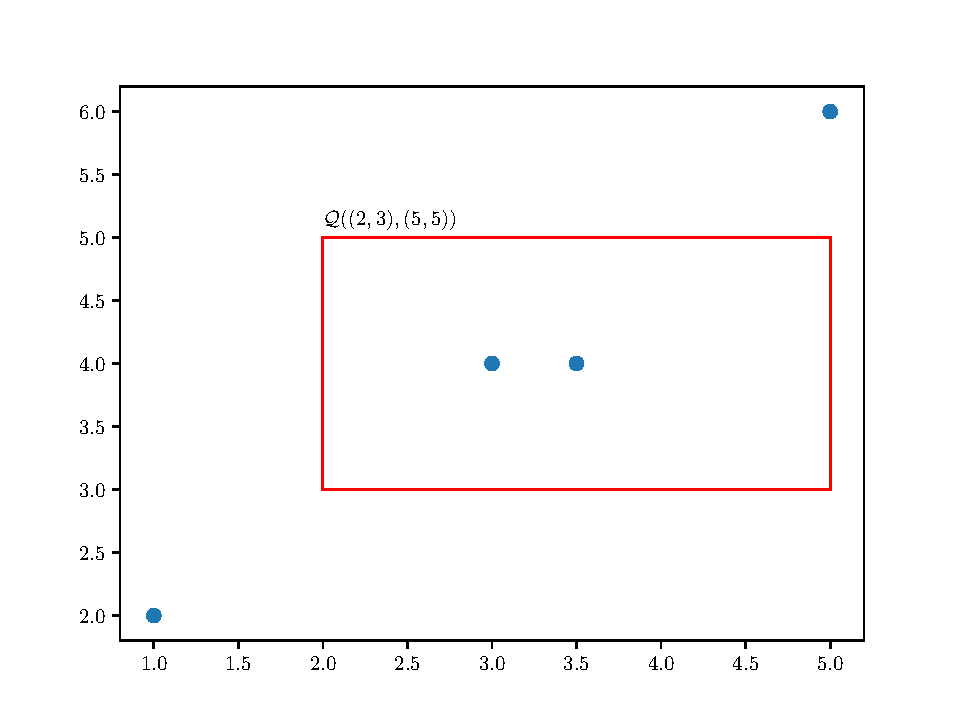
\includegraphics[width=10cm]{graphs/implementation/queries/range_query.pdf}
   	\label{fig:range_query_demo}
   	\captionof{figure}{A Range Query Example where $\mathcal{Q}(\boldsymbol{l}, \boldsymbol{u})=\mathcal{Q}((2,3),(5,5))$}
	\end{minipage}
	
In this example, the range query should return the points that lies inside the red rectangle, i.e. $[(3,4), (3.5, 4)]$.

\end{mscexample}

\subsubsection{Range Query with $K$D-Tree}

\begin{figure}[htp]
    \centering
    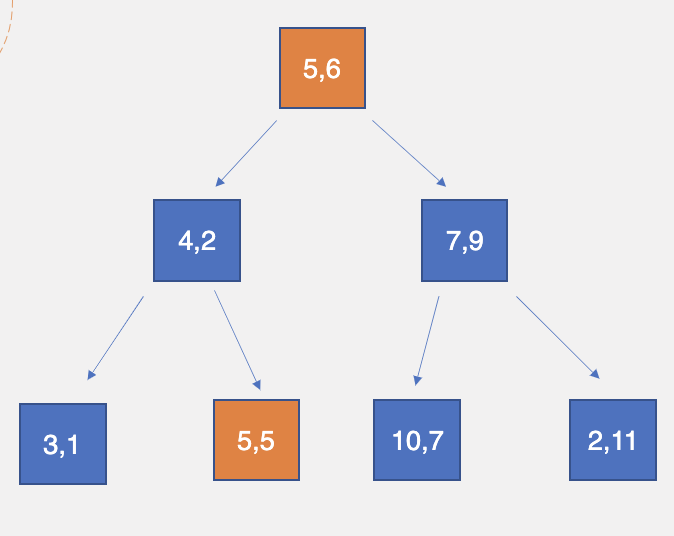
\includegraphics[width=0.4\textwidth]{graphs/Range_Query_Tree.png}
    \caption{$K$D-Tree for Range Query}
    \label{fig:KD-Tree_for_Range Query}
\end{figure}

\begin{figure}[htp]
    \centering
    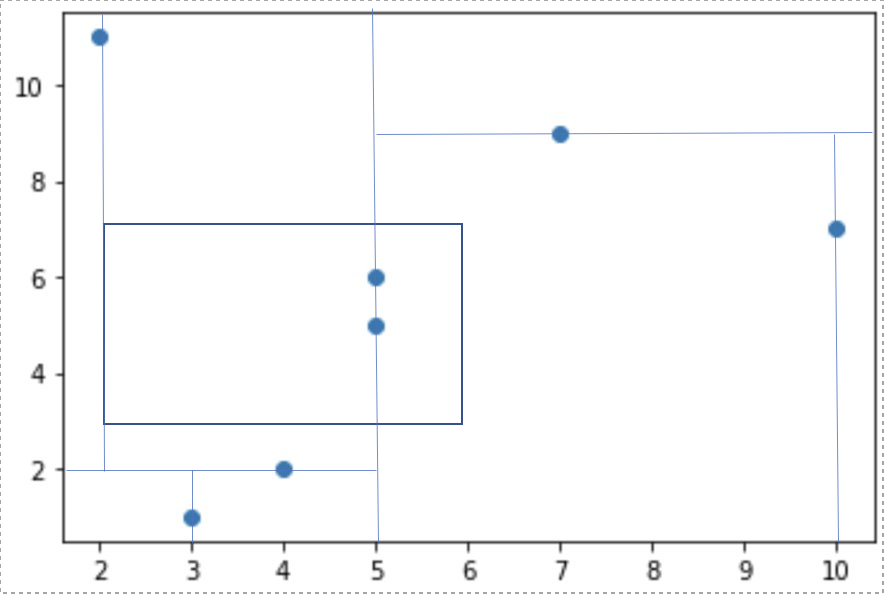
\includegraphics[width=0.6\textwidth]{graphs/Range_Query_plot.png}
    \caption{$K$D-Tree Range Query Plot on 2-dimentional plane}
    \label{fig:KD_Tree_Range_Query_Plot}
\end{figure}

% This looks very weird
We then check if the root of the tree lies within the range of the bounds and only then start traversing the tree. 

\begin{mscexample}
    For example we have a tree with Point list as 

	$$((5,6),(4,2),(7,9),(3,1),(5,5),(10,7),(2,11))$$
	
	and with lower bound = $(2,3)$ and upper bound = $(6,7)$, we will get a tree as is shown in \ref{fig:KD-Tree_for_Range Query}. We can see the points along with the rectangle range plotted in \ref{fig:KD_Tree_Range_Query_Plot}. Points $(5,5)$ and $(5,6)$ are returned in the query since they lie within the rectangle as seen in the plot. First the root point is checked and since the x-coordinate and y-coordinate both lie within the rectangle bounds i.e., $2$ > $5$ > $6$ and $3$ > $6$ > $7$. It then checks if the x-coordinate is lower than or greater than the lower bound x-coordinate. Since the value is larger than lower bound x-coordinate that is $2$ it will then traverse to the left. In the left it has child node as $(4,2)$ however, since the y-coordinate doesn't lie in the range of the upper bound this point is not selected. Therefore, it recursively traverses the tree and checks if the point lies within the bound until it reaches a leaf.
\end{mscexample}

\subsubsection{Range Query with LISA}

For a range query $\mathcal{Q}(\boldsymbol{l},\boldsymbol{u})$, we first find the cells that overlap with $\mathcal{Q}$. Then we decompose $\mathcal{Q}$ into the union of smaller query rectangles $\cap \mathcal{Q}_i$ such that each smaller query rectangles intersects only one cell.

\begin{figure*}[t]
    \centering
    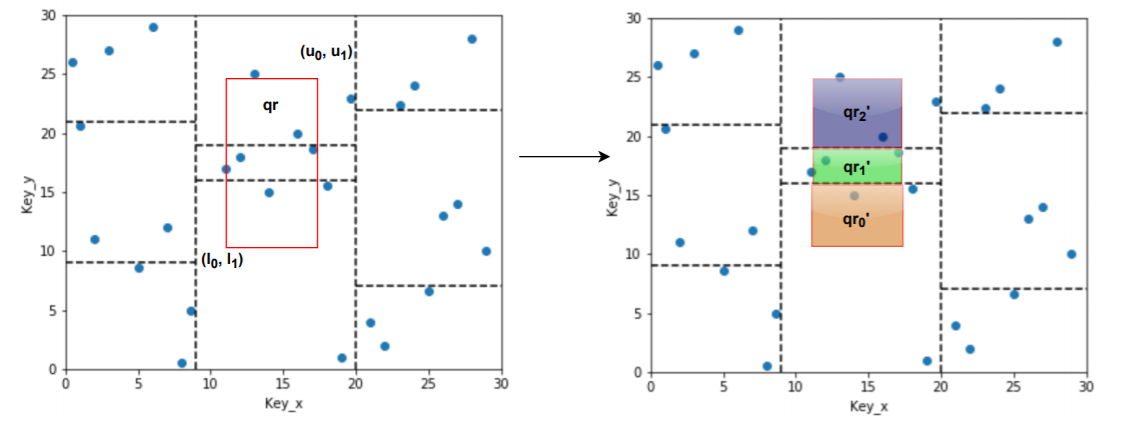
\includegraphics[width=1\textwidth]{graphs/range_query_lisa.png}
    \caption{Range Query Search in Lisa.
    1)Find the cells that overlap with query rectangle qr.    2)Decompose qr into the unions of smaller query rectangles, each of which intersect one only one cell    3)Find shards corresponding to lower and upper coordinates for each query rectangle, and perform a sequential search. }
    \label{fig:Range_Query_Lisa}
\end{figure*}

 as shown in the Fig. \ref{fig:Range_Query_Lisa}. 
 
 Suppose qr = $\bigcup\limits_{j=0}^{Q^{'}}qr_{j}^{'}$ with $qr_{j}^{'}$=$[l_{j_0}^{'},u_{j_0}^{'})\times[l_{j_1}^{'},u_{j_1}^{'}) \subseteq C_{i}$, $qr_{j}^{'}$ represents $j^{th}$ subset of range query rectangle spanning cell $C_{i}$. This is followed by calculation of mapped values of 
$qr_{j}$'s vertices. We use $m_{l}^{(0)}, m_{u}^{(0)},\cdots,m_{l}^{(Q)}, m_{u}^{(Q)}$ to denote $\mathcal{M}((l_{0_0},l_{0_1} )), \mathcal{M}((u_{0_0},u_{0_1} )), \cdots, \mathcal{M}((l_{Q_0},l_{Q_1} )), \mathcal{M}((u_{Q_0},u_{Q_1} ))$ respectively. After creating corresponding shard values,  $\mathcal{SP}(m_{l}^{0}), \mathcal{SP}(m_{u}^{0}), \cdot, \mathcal{SP}(m_{l}^{Q}), \mathcal{SP}(m_{u}^{Q})$, it is easy to select the keys that overlap with qr using sequential scan.

